\documentclass[conference]{IEEEtran}
% SBESC 2026 draft — Embedded evaluation of KAN vs MLP residual branches in
% hard-constrained recurrent physics-informed models on RISC-V.
%
% Red \tbd{...} marks results/references pending the VisionFive 2 board
% session (H1-board, H2 energy) or bibliographic verification.
% All black numbers are real, produced by the khrpinn pipeline
% (results/SUMMARY.md at the corresponding commit).

\usepackage{amsmath,amssymb}
\usepackage{booktabs}
\usepackage{graphicx}
\usepackage{multirow}
\usepackage{url}
\usepackage[table]{xcolor}
\usepackage{balance}

\newcommand{\tbd}[1]{\textcolor{red}{[TBD: #1]}}
\newcommand{\Rsq}{R^2}

\begin{document}

\title{From Discovery to Deployment: An Embedded RISC-V Evaluation of
Kolmogorov--Arnold Networks in Hard-Constrained Recurrent
Physics-Informed Models\thanks{This work was partially funded by
Funda\c{c}\~ao de Apoio da UFMG (Fundep), through Linha VI -- Conectividade
Veicular, a prioritary program from Mover (Mobilidade Verde e
Inova\c{c}\~ao), project AutoDL (29271.03.01/2023.04-00) and Auto5G
(29271.02.01/2022.01-00).}}

\author{
\IEEEauthorblockN{Enzo Nicol\'as Spotorno, Josafat Leal Filho, Ant\^onio Augusto Fr\"ohlich}
\IEEEauthorblockA{Department of Informatics and Statistics\\
Federal University of Santa Catarina, Florian\'opolis, Brazil\\
\{enzoniko, josafat, guto\}@lisha.ufsc.br}
}

\maketitle

\begin{abstract}
Hard-constrained recurrent physics-informed networks (HRPINNs) embed known
dynamics in a recurrent integrator and delegate only the unmodeled residual to
a small neural branch, making them natural candidates for real-time digital
twins on resource-constrained cyber-physical systems (CPS). Kolmogorov--Arnold
Networks (KANs) have been proposed as parameter-efficient replacements for
MLPs in such residual branches, but their learnable B-spline activations have
a fundamentally different execution profile. We present, to our knowledge, the
first systematic embedded evaluation of the vanilla B-spline KAN as an HRPINN
residual branch: a zero-dependency, scalar C++17 inference engine with
interchangeable KAN and MLP branches, bit-verified against the training
framework and deployed on a RISC-V RV64GC platform without vector extensions
(StarFive VisionFive~2, SiFive U74). Building on algorithmic results that
established when KANs match MLPs in discovery accuracy, we evaluate three
systems-level hypotheses: execution latency (H1), energy per integration step
(H2), and dependability under post-training quantization in the closed
recurrent loop (H3). On identical trained models, the KAN residual branch
executes $2.9\times$--$4.5\times$ slower than an accuracy-comparable MLP at
similar parameter count ($3.7\times$ under a deployment-optimized basis
evaluation), and exhibits input- and weight-dependent latency variation of up
to $2.2\times$ that MLPs do not show. Under INT8 quantization in the recurrent
loop, KAN trajectories diverge up to $43\times$ earlier than matched MLPs, and
attribution experiments show the dominant mechanism is per-tensor quantization
of heterogeneous spline weights rather than the often-cited grid
mis-binning. \tbd{Board latency and $\mu$J-per-step energy figures from the
VisionFive~2 measurement session.} We distill the results into deployment
guidelines for physics-informed edge CPS.
\end{abstract}

\begin{IEEEkeywords}
Kolmogorov--Arnold networks, physics-informed learning, embedded AI, RISC-V,
quantization, dependability, cyber-physical systems, digital twins
\end{IEEEkeywords}

\section{Introduction}
\label{sec:intro}

Modern cyber-physical systems increasingly rely on executable models of their
own physics --- digital twins --- for prediction, anomaly detection, and
control. When such models must run \emph{on} the system, under real-time and
energy budgets, two properties become essential: physical consistency by
construction, and a computational footprint compatible with low-cost edge
silicon. Hard-constrained recurrent architectures such as the Hybrid Recurrent
Physics-Informed Neural Network (HRPINN)~\cite{spotorno2025hard} address the
first property structurally: the known dynamics and the numerical integrator
are fixed inside the recurrent update rule, and a neural branch learns
\emph{only} the residual dynamics that the first-principles model does not
capture. This design was demonstrated to enforce physical invariants in CPS
settings and, importantly for this work, it reduces the learned component to a
small function $R_\theta:\mathbb{R}^n\!\to\!\mathbb{R}^m$ evaluated once per
integration step --- precisely the granularity at which embedded inference
cost is decided.

Kolmogorov--Arnold Networks (KANs)~\cite{liu2024kan} recently emerged as an
alternative to MLPs for scientific machine learning. Grounded in the
Kolmogorov--Arnold representation theorem, they replace fixed node activations
with learnable univariate B-splines on edges, offering an additive inductive
bias that aligns well with physical laws expressed as sums of low-order
nonlinear terms, and have shown promise for gray-box recovery of hidden terms
in dynamical systems~\cite{koenig2024kan,ma2025integrating,daryakenari2026representation,liu2025structured}.
In prior algorithmic work, summarized in Section~\ref{sec:foundations}, we
established under which conditions the \emph{vanilla} B-spline KAN matches or
loses to MLPs as an HRPINN residual branch in discovery accuracy and training
stability.\footnote{Preliminary algorithmic results were presented at a
non-archival ICLR 2026 workshop (no DOI); this paper subsumes them, adds the
embedded systems evaluation, and is the archival reference.}

Accuracy, however, is only half of the deployment equation. The literature
consistently reports that KAN inference is expensive relative to its parameter
count: recursive B-spline evaluation consumes many hardware resources, and
even LUT-based simplifications require substantial multiplexing and decoding
logic~\cite{huang2025hardware}; analytical operation counts attribute to the
original KAN formulation a several-fold multiplication overhead relative to
equally-sized MLPs~\cite{khalidHW_PLACEHOLDER}; and hardware implementations
of the basis functions are identified as a primary efficiency
burden~\cite{zhangHW_PLACEHOLDER}. Yet these observations come from
accelerator-design studies of KANs as generic classifiers/regressors. What is
missing --- and what a CPS engineer choosing a residual-branch architecture
actually needs --- is a controlled, end-to-end measurement on the deployment
class that hybrid physics-informed models target: a scalar embedded core,
inside a recurrent integrator, with the accuracy of each measured model known
on the same task. That bridge between the algorithmic result and the systems
result, on \emph{identical trained weights}, is the contribution of this
paper.

\subsection{Why this evaluation, why now, and why on these systems}
\label{sec:scope}

Three scoping decisions deserve explicit justification.

\textbf{Why the vanilla KAN.} Dozens of KAN variants (Chebyshev, wavelet,
operator-network, hybrid) now exist~\cite{mostajeran2025scaled,abueidda2025deepokan,zhang2025physics},
each claiming efficiency or stability improvements. Every one of them retains
the defining computational primitive --- per-edge univariate function
evaluation followed by summation --- and most retain B-splines. A rigorous
hardware baseline of the foundational formulation is therefore a prerequisite:
it isolates the cost of the \emph{paradigm} from the cost of any particular
engineering of it, and gives later variant evaluations a common reference
point. This mirrors standard practice in architecture research, where the
canonical algorithm is characterized before its optimized descendants.

\textbf{Why embedded in HRPINN, on a scalar RISC-V core.} The residual branch
is the only learned component of HRPINN, so the architecture comparison is
perfectly isolated: swapping $R_\theta$ changes nothing else in the
computation. HRPINN's stated purpose is dependable prediction \emph{on} CPS
platforms~\cite{spotorno2025hard}, so per-step latency and energy on edge
silicon are not an afterthought but the operating point the architecture was
designed for. We target the StarFive VisionFive~2 (SiFive U74, RV64GC): it
lacks the RISC-V vector extension, so both MLP matrix products and KAN spline
recursions compile to pure scalar instruction streams. This is deliberate:
scalar execution exposes the \emph{architectural} overhead of each topology
(operation mix, branching, locality) rather than the quality of vendor
kernels, and it is representative of the low-cost industrial SoCs where
physics-informed digital twins are expected to run. RISC-V additionally makes
the platform fully open and reproducible~\cite{visionfive2}.

\textbf{Why canonical oscillators rather than a complex industrial case
study.} We evaluate on the Duffing and Van der Pol oscillators --- the same
systems as the algorithmic study --- for four methodological reasons.
(i)~\emph{Analytical ground truth}: both residuals are known in closed form
($-0.3x^3$; $(1-x^2)v$), so discovery accuracy ($\Rsq$ against the true
residual manifold) is exactly computable, which is what allows every hardware
number in this paper to be paired with the accuracy of the very model being
measured; no real-world plant offers this. (ii)~\emph{Representative
structure}: second-order oscillatory dynamics are the canonical abstraction of
the mechanical and electrical subsystems where HRPINN-class twins apply
(suspensions, vibrating machinery, power converters, PLLs), and the pair spans
the axis that governs KAN behavior --- additively separable (Duffing) versus
multiplicative state coupling (Van der Pol). (iii)~\emph{Confound isolation}:
with a complex plant, identification error, unmodeled disturbances, and data
quality would confound hardware-induced degradation; with a controlled system,
any closed-loop divergence under quantization is attributable to the
arithmetic, which is the object of study. (iv)~\emph{A fortiori scaling}: the
per-step cost of both architectures is an explicit, exactly countable function
of layer widths (Table~\ref{tab:models}), so costs extrapolate predictably to
higher-dimensional states, while failure modes only compound --- an
architecture that misses latency, energy, or dependability targets on the
simplest two-state benchmark is disqualified for harder plants; conversely,
nothing about a larger plant removes the per-edge spline machinery measured
here. The simplification is thus conservative with respect to our
conclusions. Complex-plant case studies are the natural next step once the
architectural question is settled, and we outline them in
Section~\ref{sec:conclusion}.

\subsection{Contributions}
\begin{itemize}
\item A lightweight, zero-dependency, scalar-optimized C++17 deployment
engine for HRPINNs with interchangeable MLP and B-spline KAN residual
branches, bit-verified against the PyTorch training stack through golden-vector
test suites (35 tests / 11k checks, identical on x86-64 and RV64GC), and
released with all models, golden data, and measurement scripts.
\item A controlled latency and energy evaluation on a RISC-V RV64GC SoC,
framing and testing explicit hypotheses (H1, H2) about the scalar execution
cost of the vanilla KAN, including an anti-strawman variant with
deployment-optimized (precomputed-reciprocal) basis evaluation and analytical
operation counts for every measured model.
\item A recurrent dependability analysis (H3) of post-training static
quantization (INT16/8/6/4) inside the closed HRPINN loop, with attribution
experiments (input-, weight-, activation-only quantization) that identify
\emph{which} quantization point breaks each architecture, and a
quantized-precision extension of the discovery-accuracy metric that bridges
the algorithmic and systems results.
\item Deployment guidelines for residual-branch selection in embedded
physics-informed CPS.
\end{itemize}

\section{Background and Algorithmic Foundations}
\label{sec:foundations}

\subsection{HRPINN and the residual-learning setting}

HRPINN advances the normalized state $s_t=[x_t,v_t]$ with a hard-constrained
explicit-Euler cell,
\begin{equation}
\label{eq:cell}
\begin{aligned}
\dot v_t &= a_{\mathrm{known}}(x_t,v_t) + R_\theta(s_t),\\
x_{t+1} &= x_t + \Delta t\, v_t,\qquad
v_{t+1} = v_t + \Delta t\, \dot v_t,
\end{aligned}
\end{equation}
with $\Delta t=0.05$\,s. The known physics $a_{\mathrm{known}}$ and the
integrator are fixed; only $R_\theta$ is trained, either by one-step teacher
forcing (TF) or by backpropagation through time (BPTT) over 20-step windows.
The residual branch is implemented either as a ReLU MLP or as a vanilla
B-spline KAN~\cite{liu2024kan} (grid size $G{=}5$, order $k{=}3$ unless
stated; SiLU base path plus spline path, with training-adaptive, generally
non-uniform grids). Benchmark systems: Duffing
($\dot v = -x -0.2v -0.3x^3$, known part $-x-0.2v$, residual $-0.3x^3$) and
Van der Pol ($\dot v = -x + (1-x^2)v$, known part $-x$, residual $(1-x^2)v$).
Discovery accuracy is the $\Rsq$ between the learned surface
$R_\theta(x,v)$ and the analytical residual on a $50\times50$ grid over
$[-2,2]^2$.

\subsection{Summary of algorithmic findings}
\label{sec:algofindings}

Our preliminary study (100 seeds per configuration) established four
behaviors of the vanilla KAN in this setting, condensed in
Table~\ref{tab:iclr}:
(i)~small KANs match or exceed similarly sized MLPs on the separable
univariate Duffing residual;
(ii)~KANs consistently fail to accurately recover the multiplicative Van der
Pol interaction, where MLPs scale gracefully;
(iii)~KAN performance is fragile with respect to grid size, sparsity
regularization, and update schedule, with several configurations yielding
negative $\Rsq$, a sensitivity absent in MLPs~\cite{noorizadegan2025practitioner};
(iv)~deeper KAN configurations are unstable under recurrent (BPTT)
optimization~\cite{sohail2024training}.
These results pose the systems question this paper answers: \emph{does the
parameter efficiency KANs exhibit on separable residuals translate into
computational efficiency on edge hardware, or does the B-spline formulation
introduce execution- and precision-level costs that negate it?}

\begin{table}[t]
\centering
\caption{Algorithmic baseline (BPTT recipe): Discovery $\Rsq$, mean $\pm$95\%
CI over 100 seeds, from the preliminary study. Params as in
Table~\ref{tab:models}.}
\label{tab:iclr}
\small
\begin{tabular}{llcc}
\toprule
Arch. & Config. & Duffing $\Rsq$ & Van der Pol $\Rsq$ \\
\midrule
\multirow{4}{*}{KAN}
 & Very Small & $0.914\pm0.061$ & $0.743\pm0.061$ \\
 & Small      & $0.874\pm0.080$ & $0.785\pm0.073$ \\
 & Wide       & $0.468\pm0.773$ & $-0.602\pm2.842$ \\
 & Deep       & (unstable)      & $0.754\pm0.079$ \\
\midrule
\multirow{4}{*}{MLP}
 & Tiny   & $0.906\pm0.092$ & $0.622\pm0.173$ \\
 & Small  & $0.937\pm0.047$ & $0.879\pm0.032$ \\
 & Medium & $0.951\pm0.033$ & $0.879\pm0.019$ \\
 & Large  & $0.932\pm0.063$ & $0.898\pm0.017$ \\
\bottomrule
\end{tabular}
\end{table}

\section{Embedded Inference Framework}
\label{sec:framework}

\subsection{Engine design}

We implement both residual branches and the HRPINN cell
(Eq.~\ref{eq:cell}) in a dependency-free C++17 engine (libc/libm only,
statically linked for minimal Linux images). Both branches are
allocation-free, cache-contiguous scalar loops: the MLP is a chain of fused
GEMV+ReLU passes over row-major weights; the KAN evaluates, per input feature,
the SiLU base path and the Cox--de~Boor recursion over that feature's
(generally non-uniform, training-adapted) knot vector, followed by the spline
GEMV with the per-edge scaler pre-folded into the spline weights at export.
Models are exported from PyTorch into a compact binary format carrying
weights, knot vectors, the normalizer, the integrator step, and per-tensor
calibration ranges.

Two implementation choices matter for fairness. First, the default KAN path
reproduces the reference PyTorch numerics operation-for-operation (explicit
divisions by knot differences), which lets us pin the engine against the
training framework; a second, deployment-optimized path multiplies by
reciprocals precomputed at load time (the grid is frozen at inference) and is
reported alongside it, so the KAN is measured at its best plausible scalar
implementation. Second, both architectures receive identical treatment in
every other respect: same compiler and flags (\texttt{-O2},
\texttt{-ffp-contract=off}), single thread, same measurement harness.

\subsection{Verification methodology}
\label{sec:verification}

Because a hardware evaluation is only as sound as the equivalence between the
measured binary and the published algorithm, the engine is pinned to the
training stack by golden-vector suites generated from the trained PyTorch
models: 256 branch inputs per model (uniform, spline-knot-boundary,
out-of-domain, and on-trajectory states), 64 single cell steps, and three
500-step closed-loop rollouts. The FP32 engine matches PyTorch within
$10^{-4}$ relative on all 20 exported models and within $5\times10^{-3}$
normalized state error over full rollouts; the MLP path is bit-identical to a
NumPy reference. The quantized engine (below) is pinned within one
quantization LSB against an independent Python implementation of the same
specification. The full suite (35 tests, $\approx$11k checks) passes
identically when cross-compiled to RV64GC and executed under
\texttt{qemu-riscv64}, and integer-path outputs are bit-exact across x86-64
and RISC-V; the board workflow re-runs the golden verification on-device
before any measurement.

\subsection{Post-training quantization strategy}
\label{sec:quant}

We implement post-training \emph{static} quantization in its baseline form,
deliberately without KAN-specific co-design (which prior work indicates is
necessary to keep KAN accuracy losses below fractions of a
percent~\cite{huang2025hardware}): symmetric per-tensor weight quantization
($\mathrm{scale}=\max|w|/q_{\max}$), affine per-tensor activation and state
quantization calibrated from min/max ranges over the training trajectories,
at INT16, INT8, and (as additional degradation data points) INT6 and INT4.
Execution follows the standard simulated-integer model: values are stored
with intN semantics and dequantized for float arithmetic at tensor
boundaries; the B-spline bin search consumes the truncated (dequantized)
input, reproducing the mis-binning mechanism hypothesized in the literature.
MLP biases remain exact, as int32 biases are in real integer pipelines.
Consequently, quantized configurations are evaluated for \emph{accuracy and
stability} (H3), not speed: we make no latency claims about integer execution.
Five quantization modes allow attribution: \texttt{full} (state, weights and
activations, with the recurrent state requantized every step, as a fully
integer sensor-to-actuator loop would), \texttt{residual\_only} (float loop,
quantized branch), and \texttt{input}-, \texttt{weights}-, and
\texttt{activations}-only.

\begin{table}[t]
\centering
\caption{Evaluated residual branches (identical trained weights in Python and
C++; median-of-5-seeds export). Ops = scalar FLOPs per branch inference
(analytical); exp = transcendental calls. Weights incl.\ knot vectors, FP32.}
\label{tab:models}
\small
\setlength{\tabcolsep}{4.5pt}
\begin{tabular}{llrrrr}
\toprule
Arch. & Config. & Layers & Params & Ops (+exp) & Bytes \\
\midrule
\multirow{4}{*}{KAN}
 & Very Small & [2,4,1]   & 120  & 1350 (+6)  & 720 \\
 & Small      & [2,8,1]   & 240  & 2322 (+10) & 1344 \\
 & Wide       & [2,16,1]  & 480  & 4266 (+18) & 2592 \\
 & Deep       & [2,8,8,1] & 880  & 4986 (+18) & 3904 \\
\midrule
\multirow{4}{*}{MLP}
 & Tiny   & [2,8,8,1]    & 105  & 209  & 420 \\
 & Small  & [2,16,16,1]  & 337  & 673  & 1348 \\
 & Medium & [2,32,32,1]  & 1185 & 2369 & 4740 \\
 & Large  & [2,64,64,1]  & 4417 & 8833 & 17668 \\
\bottomrule
\end{tabular}
\end{table}

\section{Hypotheses and Embedded Evaluation}
\label{sec:eval}

\subsection{Setup}

All 8 configurations of Table~\ref{tab:models} are trained per system
(Duffing, Van der Pol) with the BPTT recipe of the algorithmic study (5 seeds;
the \emph{median} seed by discovery $\Rsq$ is exported, avoiding
cherry-picking), yielding 16 primary models plus 4 TF-trained KAN reference
configurations. Latency uses a pinned single core, $10^4$ warmup calls, and 3
interleaved rounds of 10 repetitions $\times\,10^5$ calls over a fixed buffer
of 1024 states, with checksum sinks preventing dead-code elimination; we
report medians. Development-host numbers (x86-64, Zen; gcc 13.3) are reported
to characterize the architectures; the RISC-V numbers
(VisionFive~2, U74 @ 1.5\,GHz, gcc 13.3 cross, identical flags) are the
paper's headline platform. \tbd{Board latency table pending measurement
session; procedure and pre-verified binaries are frozen in the artifact.}

\subsection{H1: Execution latency}
\label{sec:h1}

\textbf{Hypothesis.} Despite its lower parameter count at comparable Duffing
accuracy, the KAN residual branch incurs substantially higher per-step latency
than the MLP in scalar execution.

\textbf{Rationale.} Per branch inference, an MLP layer costs $n_{in}n_{out}$
multiply--accumulates; a KANLinear layer costs a base GEMV
($n_{in}n_{out}$), $n_{in}$ SiLU evaluations (each one \texttt{expf}), the
per-feature Cox--de~Boor recursion ($\mathcal{O}((G{+}2k)k)$ data-dependent
operations including divisions), and a spline GEMV
($n_{in}n_{out}(G{+}k)$)~\cite{khalidHW_PLACEHOLDER,huang2025hardware}.
Table~\ref{tab:models} makes this concrete: at comparable parameter count
(KAN Very Small vs.\ MLP Tiny), the KAN executes $6.5\times$ the scalar
operations plus transcendentals.

\begin{table}[t]
\centering
\caption{H1 --- residual-branch latency (ns/call, median). ``recip'' = KAN
with precomputed-reciprocal basis path. Board column measured on the
VisionFive~2. PC: x86-64, gcc 13.3, \texttt{-O2}, single core.}
\label{tab:latency}
\small
\setlength{\tabcolsep}{4pt}
\begin{tabular}{llrrrr}
\toprule
Arch. & Config. & Params & PC & PC recip & U74 (board) \\
\midrule
\multirow{4}{*}{KAN}
 & Very Small & 120 & 244 & 203 & \tbd{ns} \\
 & Small      & 240 & 428 & 372 & \tbd{ns} \\
 & Wide       & 480 & 763 & 658 & \tbd{ns} \\
 & Deep       & 880 & 882--2033$^{\dagger}$ & 780--1863$^{\dagger}$ & \tbd{ns} \\
\midrule
\multirow{4}{*}{MLP}
 & Tiny   & 105  & 54   & --- & \tbd{ns} \\
 & Small  & 337  & 146  & --- & \tbd{ns} \\
 & Medium & 1185 & 414--484$^{\ddagger}$ & --- & \tbd{ns} \\
 & Large  & 4417 & 1549--1712$^{\ddagger}$ & --- & \tbd{ns} \\
\bottomrule
\multicolumn{6}{l}{\footnotesize $^{\dagger}$range across the two systems'
trained weights (see text); $^{\ddagger}$minor spread.}
\end{tabular}
\end{table}

\textbf{Results (development host; board pending).}
Table~\ref{tab:latency} confirms the hypothesis on scalar x86: at comparable
parameter count, KAN Very Small (120 params) takes 244\,ns per call against
54\,ns for MLP Tiny (105 params) --- $4.5\times$ --- and KAN Small (240) takes
$2.9\times$ the latency of the more accurate MLP Small (337). The
deployment-optimized reciprocal path recovers 6--18\% (median 15\%), still
leaving a $3.7\times$ gap at matched size; the conclusion is robust to
implementation effort. Normalized differently: the KAN spends
$\approx$2.0\,ns per parameter versus $\approx$0.4\,ns for MLPs, so the
parameter-efficiency argument inverts at execution time. Two further
observations strengthen the mechanism account. First, MLP latency tracks its
operation count almost perfectly across three orders of magnitude
(Table~\ref{tab:models} vs.~\ref{tab:latency}), while KAN latency per
operation is consistently higher, reflecting the recursion's data-dependent
branching and non-contiguous accesses. Second, KAN latency is
\emph{weight- and input-dependent}: the two Deep KANs --- architecturally
identical, differing only in trained weights and adapted grids --- differ by
$2.2\times$ (882 vs.\ 2033\,ns), a variance MLPs do not exhibit ($<$10\%) and
itself a liability for worst-case execution-time analysis in real-time CPS.
\tbd{Confirm ratios and the data-dependent effect on the U74; expectation
from the in-order pipeline is equal or larger gaps.}

Full accuracy--latency Pareto fronts (every model of Table~\ref{tab:iclr}
against its measured latency) are provided in the artifact; MLPs dominate the
front everywhere except the extreme low-memory corner on Duffing, preempting
the objection that KANs would win at equal \emph{accuracy} rather than equal
parameters.

\subsection{H2: Energy per integration step}
\label{sec:h2}

\textbf{Hypothesis.} The KAN branch consumes disproportionately more energy
per HRPINN step ($\mu$J) than the accuracy-comparable MLP.

\textbf{Rationale.} On a single in-order core at fixed frequency, energy per
step is dominated by active-power $\times$ latency; H1's latency gap should
therefore reproduce in energy, amplified if the KAN's branchy, less
cache-regular execution also raises average active power (pipeline stalls
keep the core busy without retiring work)~\cite{zhangHW_PLACEHOLDER}.

\textbf{Protocol.} Board powered through an inline USB-C power meter;
differential measurement (idle power subtracted from steady-state power during
a 120\,s fixed-duration step loop, with the loop's measured steps/s), so that
$\mu\mathrm{J/step} = (P_{\mathrm{load}}-P_{\mathrm{idle}})/(\mathrm{steps/s})$.
Governor pinned, idle re-measured at session end ($\pm3\%$ drift bound). The
complete pipeline (loop binary, log format, aggregation) is frozen and was
validated end-to-end in a dry run; only the meter readings are pending.

\textbf{Expected/observed results.} \tbd{Energy table ($\mu$J/step for all 8
configurations $\times$ 2 systems), measured on the VisionFive~2. Expected
from H1: KAN $\mu$J/step exceeding matched MLPs by at least the latency
ratio; report whether average active power also differs, which would indicate
microarchitectural (stall-driven) amplification beyond the latency effect.}

\subsection{H3: Recurrent dependability under quantization}
\label{sec:h3}

\textbf{Hypothesis.} Under baseline INT8 post-training quantization inside
the closed recurrent loop, KAN branches lose trajectory fidelity
catastrophically earlier than matched MLPs, whereas INT16 is safe for both.

\textbf{Rationale.} KANs depend on precise positioning of inputs within
spline grid intervals, and their per-edge functions have heterogeneous ranges
that share single per-tensor scales under baseline PTQ; prior work reports
that keeping KAN quantization losses small requires dedicated co-design
techniques~\cite{huang2025hardware}. In a recurrent integrator, any such
localized error is fed back and compounds across steps.

\textbf{Protocol.} For every model: 20 initial conditions, 2000-step
(100\,s) closed-loop rollouts at FP32/INT16/INT8/INT6/INT4 in \texttt{full}
and \texttt{residual\_only} modes plus the three single-point attribution
modes at INT8; per-step error is the normalized-state $L_2$ distance to the
same model's FP32 rollout (isolating quantization from model error);
divergence is the first crossing of $0.1$. Deterministic and bit-reproducible
across hosts, so PC results are authoritative;
\tbd{two on-board spot checks demonstrating bit-equality, per runbook}.

\begin{table}[t]
\centering
\caption{H3 --- closed-loop divergence (\texttt{full} mode): fraction of 20
ICs diverged / median divergence step (2000 = horizon, ``---'' = never).
Matched accuracy-comparable pairs grouped.}
\label{tab:dependability}
\small
\setlength{\tabcolsep}{4.2pt}
\begin{tabular}{llrrrr}
\toprule
& & \multicolumn{2}{c}{INT16} & \multicolumn{2}{c}{INT8} \\
\cmidrule(lr){3-4}\cmidrule(l){5-6}
System & Model & div. & step & div. & step \\
\midrule
\multirow{4}{*}{Duffing}
 & KAN Very Small & 0\,\%   & --- & 100\,\% & \textbf{6.5} \\
 & MLP Tiny       & 0\,\%   & --- & 100\,\% & 282 \\
 & KAN Small      & 0\,\%   & --- & 100\,\% & 119 \\
 & MLP Small      & 0\,\%   & --- & 100\,\% & 316 \\
\midrule
\multirow{4}{*}{Van der Pol}
 & KAN Very Small & 0\,\%   & --- & 100\,\% & 78 \\
 & MLP Tiny       & 0\,\%   & --- & 100\,\% & 196 \\
 & KAN Small      & 100\,\% & 575 & 100\,\% & 93 \\
 & MLP Small      & 0\,\%   & --- & 100\,\% & 146 \\
\bottomrule
\end{tabular}
\end{table}

\textbf{Results.} Table~\ref{tab:dependability} confirms the hypothesis with
an important refinement. At INT16, all matched small models remain within
tolerance for the full 100\,s horizon (the only failures anywhere at INT16 are
KAN configurations already flagged as fragile in Table~\ref{tab:iclr}). At
INT8 in \texttt{full} mode --- where the state itself is requantized each step
--- \emph{every} model eventually crosses the threshold, because 8-bit state
resolution ($2/255$ of the normalized range) accumulates in any recurrent
integrator; the architectures differ radically in \emph{when}: the Duffing
KAN Very Small collapses at a median of 6.5 steps (0.3\,s) versus 282 steps
(14\,s) for the matched MLP --- $43\times$ earlier --- with the same ordering
across all matched pairs. \texttt{residual\_only} mode (float loop, quantized
branch) removes the state-truncation floor and preserves the gap: KAN Small
diverges at a median step 137 versus 1183 for MLP Small on Duffing, and the
best small MLP never diverges where its KAN counterpart fails within seconds.

\begin{table}[t]
\centering
\caption{H3 attribution at INT8 (Duffing, matched pair): median trajectory
MSE vs.\ FP32 rollout when quantizing only one component.}
\label{tab:attribution}
\small
\begin{tabular}{lrr}
\toprule
Quantized component & KAN Very Small & MLP Tiny \\
\midrule
input only          & $3\times10^{-6}$ & $2\times10^{-6}$ \\
weights only        & $0.204$          & $6\times10^{-5}$ \\
activations only    & $0.048$          & $2\times10^{-5}$ \\
full loop           & $0.275$          & $4\times10^{-3}$ \\
\bottomrule
\end{tabular}
\end{table}

\begin{figure*}[t]
\centering
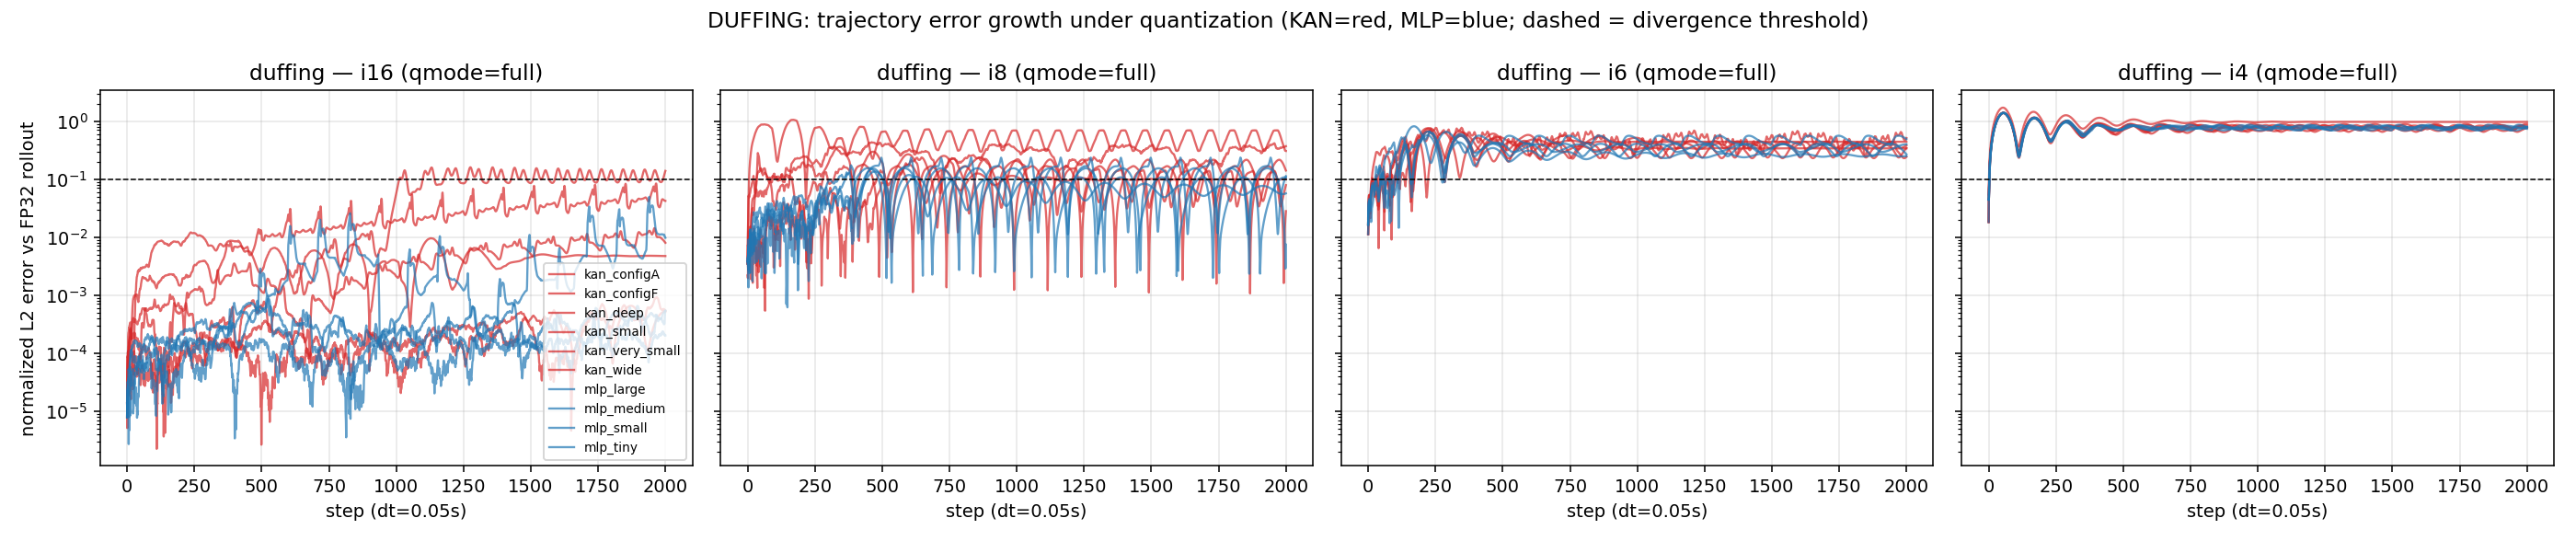
\includegraphics[width=\textwidth]{../results/figures/degradation_duffing.png}
\caption{Trajectory error growth under quantization (Duffing, \texttt{full}
mode, error vs.\ the same model's FP32 rollout; KAN models red, MLP blue;
dashed line = divergence threshold). INT16 keeps all models within tolerance;
at INT8 the KANs cross the threshold one to two orders of magnitude earlier
than matched MLPs; INT6/INT4 destroy both. \tbd{Re-render with final styling
and the Van der Pol panel if page budget allows.}}
\label{fig:degradation}
\end{figure*}

\textbf{Mechanism.} The attribution experiment (Table~\ref{tab:attribution})
overturns the most commonly cited explanation. Quantizing \emph{only the
input} --- the grid mis-binning mechanism --- is essentially harmless to both
architectures: at INT8 the input step ($\approx0.008$) is $50\times$ smaller
than a spline bin ($0.4$). The damage comes from \emph{weight} quantization
(KAN trajectory MSE $0.204$ vs.\ $6\times10^{-5}$ for the MLP: three orders of
magnitude) and secondarily from activations. The cause is structural: a
KANLinear layer concentrates most parameters in one spline-coefficient tensor
whose per-edge sub-functions have heterogeneous magnitudes, so a single
per-tensor scale crushes the small coefficients that shape individual basis
segments; the MLP's homogeneous weight matrices tolerate the same scheme.
This redirects mitigation: per-edge (per-channel) spline-weight scales, not
finer input grids, are the co-design KANs need --- consistent with the
hardware-aware quantization emphasis of~\cite{huang2025hardware}.

\textbf{Bridge to the discovery metric.} Recomputing the algorithmic study's
discovery $\Rsq$ through the quantized engine collapses the two papers'
metrics into one table: on Duffing, KAN Very Small falls from $\Rsq=0.90$
(FP32) to $-0.10$ at INT8 while MLP Tiny degrades from $0.95$ to $0.92$;
KAN Deep falls to $-0.20$ while MLP Medium retains $0.94$. On Van der Pol,
both architectures degrade mildly at INT8 ($\leq0.02$), showing the collapse
is not universal but weight-distribution-dependent --- reinforcing the
per-tensor-scale mechanism. Error-growth curves for all models and precisions
are in the artifact.

\section{Deployment Guidelines for Embedded Physics-Informed CPS}
\label{sec:guidelines}

\begin{enumerate}
\item \textbf{Default to MLP residual branches} for dependable edge
deployment: at matched accuracy they are faster (H1), \tbd{more
energy-efficient (H2, pending board numbers)}, latency-deterministic, and
degrade gracefully under baseline quantization (H3).
\item \textbf{Reserve vanilla KANs for the low-memory, additive-physics
corner}: FP32 or INT16 execution, strictly separable residual structure,
generous real-time margins (their latency is weight- and input-dependent),
and no INT8 pipelines without KAN-specific quantization co-design.
\item \textbf{Quantize the loop, not just the network, in your analysis}: in
\texttt{full}-integer loops even well-behaved MLPs accumulate state-truncation
error (all INT8 rollouts eventually drift); dependability budgets must be set
against horizon-specific divergence times, which our protocol measures
directly.
\item \textbf{If KANs must be quantized}, prioritize per-edge spline-weight
scales over input-grid precision --- our attribution data shows the
per-tensor weight scale, not bin mis-assignment, is the failure driver.
\end{enumerate}

\section{Threats to Validity}
\label{sec:threats}

\textbf{Internal.} The engine is pinned to the training framework by golden
tests (Section~\ref{sec:verification}); measurement noise is bounded by
interleaved rounds and reported percentiles. The KAN is measured at both the
reference-faithful and a deployment-optimized basis implementation, bounding
implementation bias at $\leq$18\%. Exported models are median-of-5 seeds.
\textbf{Construct.} Quantized execution is simulated-integer (standard PTQ
semantics); we therefore make no claims about integer \emph{latency}, only
about precision-induced behavior, which the simulation reproduces exactly by
construction. Energy is measured differentially at the board input, capturing
SoC+DRAM but not isolating the core --- appropriate for system-level
budgeting. \textbf{External.} Two canonical two-state plants and one scalar
RV64GC core; Section~\ref{sec:scope} argues why this is the right controlled
setting and in which direction each simplification is conservative.
Generalization to vectorized cores (RVV, NEON) is explicitly out of scope:
vector units would change both architectures' constants, though the KAN's
gather-heavy, branchy recursion vectorizes worse than GEMV in principle.

\section{Conclusion and Future Work}
\label{sec:conclusion}

We bridged an algorithmic result --- when vanilla KANs match MLPs as
hard-constrained residual learners --- to its systems consequence on open
embedded hardware, with a verified, released pipeline in which every measured
binary is provably the published algorithm. The parameter efficiency of the
vanilla KAN does not survive deployment scrutiny: at matched accuracy and
parameter budget it executes several times slower under scalar execution,
with weight-dependent timing variance, and its quantization robustness in the
recurrent loop is dominated by a structural weakness (per-tensor spline-weight
scales) that baseline PTQ cannot accommodate --- while MLPs remain fast,
deterministic, and gracefully degrading. \tbd{One-sentence quantitative
summary of board latency and energy once measured.}

Future work follows three axes: (i) evaluating KAN variants and co-designed
quantization (per-edge scales, LUT-based basis evaluation,
CIM-style analog activation generation~\cite{wenCIM_PLACEHOLDER,huang2025hardware})
against this baseline; (ii) scaling the dependability methodology to
higher-dimensional and eventually industrial plants (vehicle dynamics,
power-electronics twins) now that the architectural variables are
characterized in isolation; (iii) vectorized (RVV) implementations to test
whether the scalar gap narrows or widens with data-level parallelism.

\balance
\bibliographystyle{IEEEtran}
\bibliography{references}

\end{document}
